\section{Evaluating Models} \label{evalmodels}
%\todo{shorten this}

A number of different machine learning algorithms were used, and the \textit{accuracy} for each model was calculated as an estimate for it's overall performance. Accuracy is defined to be the proportion of correctly predicted instances to the total number of predictions:

\begin{equation}
    accuracy = \frac{tp+tn}{tp+tn+fp+fn}
\end{equation}

where $tp$ and $tn$ are true positives and true negatives, and $fp$ and $fn$ are false positives and false negatives respectively \cite{vanwinckelen2012estimating}. Confusion matrices for each classification model can be visualised in Figure \ref{confusionmatricesr2}.
%\sophie{should figures 2 and 3 be kept?}
%\denes{No, but we could report all the confusion matrices for each model (possibly in the appendices).}
Additionally, precision and recall were calculated for each model.
%Precision is defined as the proportion of true positives to the total number of predictions predicted positive, and is a percentage of returned results which are relevant. Recall is defined to be the proportion of true positives to the total number of actual positives, and is a percentage of relevant data which have been correctly classified \cite{buckland1994relationship}.

\begin{equation}
    precision = \frac{tp}{tp+fp} \\
\quad recall = \frac{tp}{tp+fn}
\end{equation}

Both metrics are important to take into consideration, and ultimately we use the F1 measure, which can be interpreted as the harmonic mean between precision and recall \cite{buckland1994relationship}, and accuracy score for evaluation of each classifier.

\begin{equation}
    F1 \ score = 2 \cdot \frac{precision \cdot recall}{precision + recall}
\end{equation}

An issue associated with training models is the possibility for the model to \textit{overfit}. We use cross validation in order to limit overfitting.
%Overfitting occurs when a model captures unwanted bias and noise in the data that it negatively impacts the performance of a model. The model corresponds to it's initial training data too well, and fails to predict unseen data reliably. In order to limit overfitting, a popular re-sampling technique called $k$-fold cross validation is used.
In cross validation, the dataset is split into $k$ random subsets, known as folds, and one is selected as a test set for the model to test on, while the others are used as a training set for the model to train on. This is repeated $k$ times where a different subset of data is used as the test set each time, and the overall performance of the model is calculated as the average of accuracy scores for each iteration \cite{berrar2019cross}.

\section{Experimental Results} \label{experresults}
The whole dataset was split in a ratio such that there was a training set, validation set and test set in a 18:72:10 ratio. 10\% of the original dataset was used as a test set, and of the remaining 90\%, the data was split in an 80:20 ratio for the training and validation set.
The model trains on the training set, and the validation set is used for optimising the hyperparameters of the model.
The test set is completely left out from the training process of the model, and is only used during evaluation. This is to see how well models generalise to unseen data which replicate new match data, as the test set is never used before evaluation. During evaluation, all other data is used for training the model (training and validation).
Both accuracy and F1 score is reported for the validation and test sets. The standard deviation for each score for the validation set is reported as a basis of defining uncertainty; the results are shown in Table \ref{results}.

\begin{table}[H]
\caption{Model performance comparing validation and test sets}
\label{results}
\centering
\setlength{\tabcolsep}{3pt}
\scalebox{1.05}{%
\begin{tabular}{ l|c c|c c }

\multirow{2}{4em}{Model} &
\multicolumn{2}{|c|}{Validation set} &
\multicolumn{2}{|c}{Test set} \\
\cline{2-5}
  & Acc & F1 & Acc & F1 \\

\hline \hline 
Logistic Regression & 0.699$\pm{0.053}$ & 0.705$\pm{0.052}$ & 0.722 & 0.706 \\
Random Forest & 0.677$\pm{0.071}$ & 0.688$\pm{0.073}$ & 0.667 & 0.684 \\
Support Vector Machine & & \\
$\rightarrow$ Linear & 0.696$\pm{0.064}$ & 0.690$\pm{0.078}$ & 0.639 & 0.629 \\
$\rightarrow$ RBF    & 0.700$\pm{0.056}$ & 0.677$\pm{0.077}$ & 0.667 & 0.600 \\
$\rightarrow$ Polynomial & 0.705$\pm{0.046}$ & 0.685$\pm{0.046}$ & 0.611 & 0.563\\
$\rightarrow$ Sigmoid & 0.705$\pm{0.039}$ & 0.690$\pm{0.041}$ & 0.694 & 0.621 \\
MLP Neural Network & 0.696$\pm{0.043}$ & 0.708$\pm{0.045}$ & 0.694 & 0.703\\
[1ex]
\hline
\end{tabular}}
\end{table}

Receiving operating characteristics (ROC) learning curves and the trade-off between precision and recall can be seen from Figures \ref{roc} and \ref{par}. ROC curves demonstrate the performance of a classification model for all classification thresholds. The closer the apex of the curve is to the upper left hand corner, the greater the model's discriminatory ability \cite{fan2006understanding}. This is plotted for each type of classifier, including the SVM model using a linear kernel. 
For each trained model, we use it's accuracy score, F1 measure and the area under it's ROC curve to evaluate overall performance.

\begin{figure}[ht]
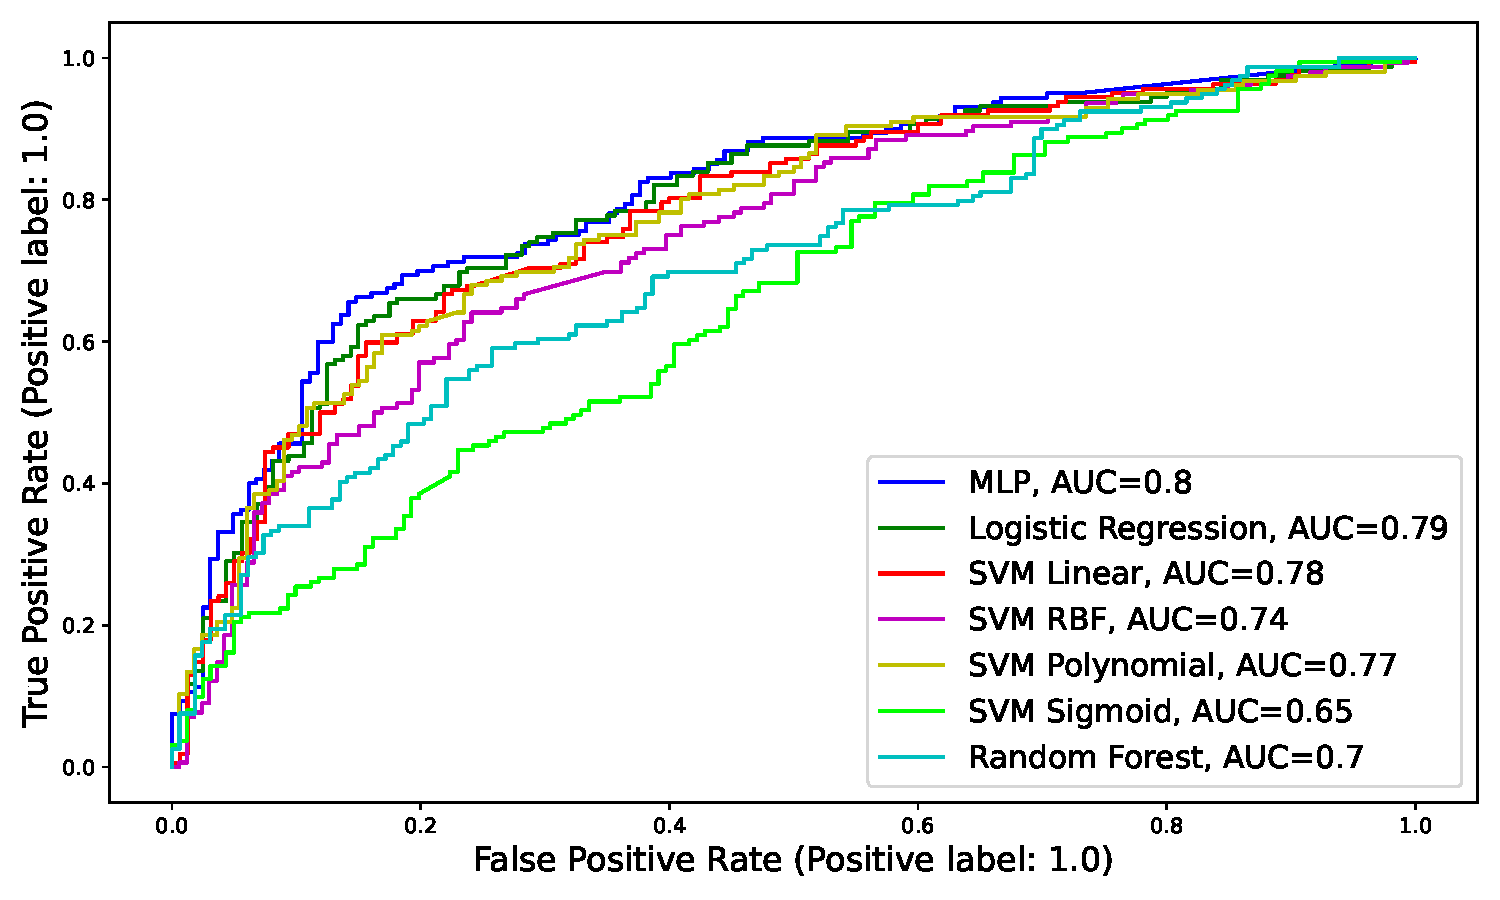
\includegraphics[width=8.5cm]{plots/roccurves.pdf}
\caption{ROC Learning Curves}

\label{roc}
\centering
\end{figure}

\begin{figure}[ht]
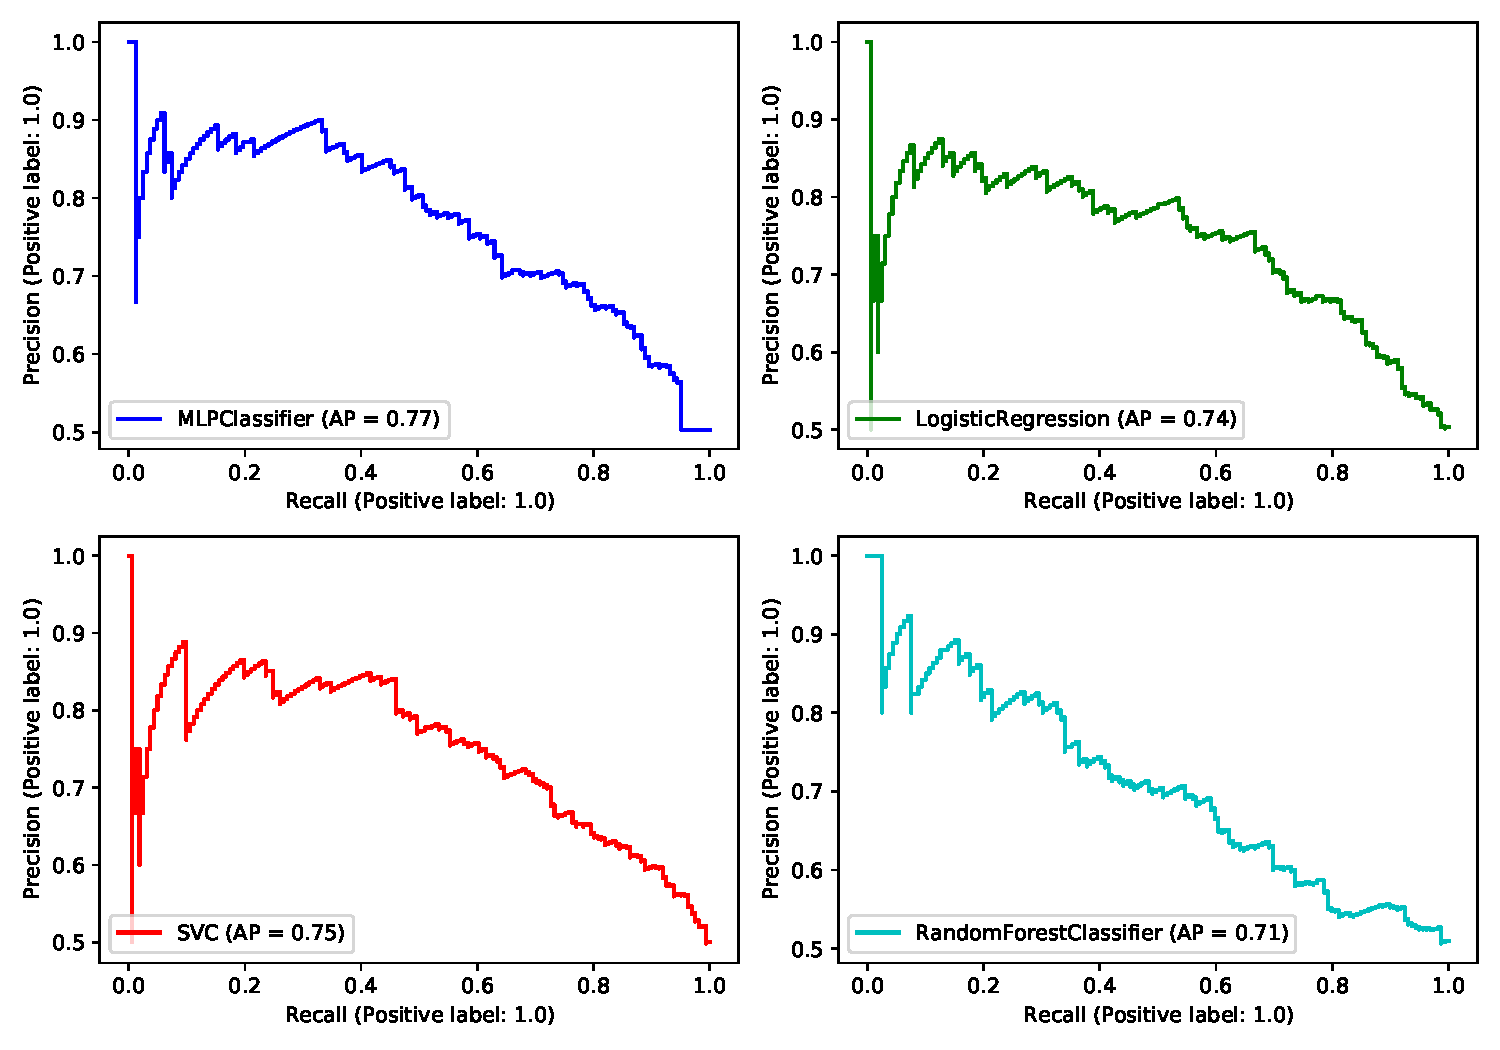
\includegraphics[width=8.5cm]{plots/precisionrecall.pdf}
\caption{Precision and Recall Curves}

\label{par}
\centering
\end{figure}

